\chapter{Data Analysis and Results}



%-------------------------
%        RAW DATA
%-------------------------
\section{Raw Data}
The raw data consisted of a total of 7 videos and are laid out in \refFig{datacollection}. Barrier height, acceleration of the tray, Faraday threshold, and percentage of ``transmissions" were recorded for each of the 7 videos. The 7 videos contained: one trial of a single droplet for all three barrier heights, another trial of a single droplet for all three barrier heights, and a final trial of a single droplet for the $3.0~\mathrm{mm}$ barrier. The same droplet was used for each of the three barrier heights in a trial. There were between 12 to 24 separate collisions for each barrier. 

\begin{figure}[h!]
	\centering
	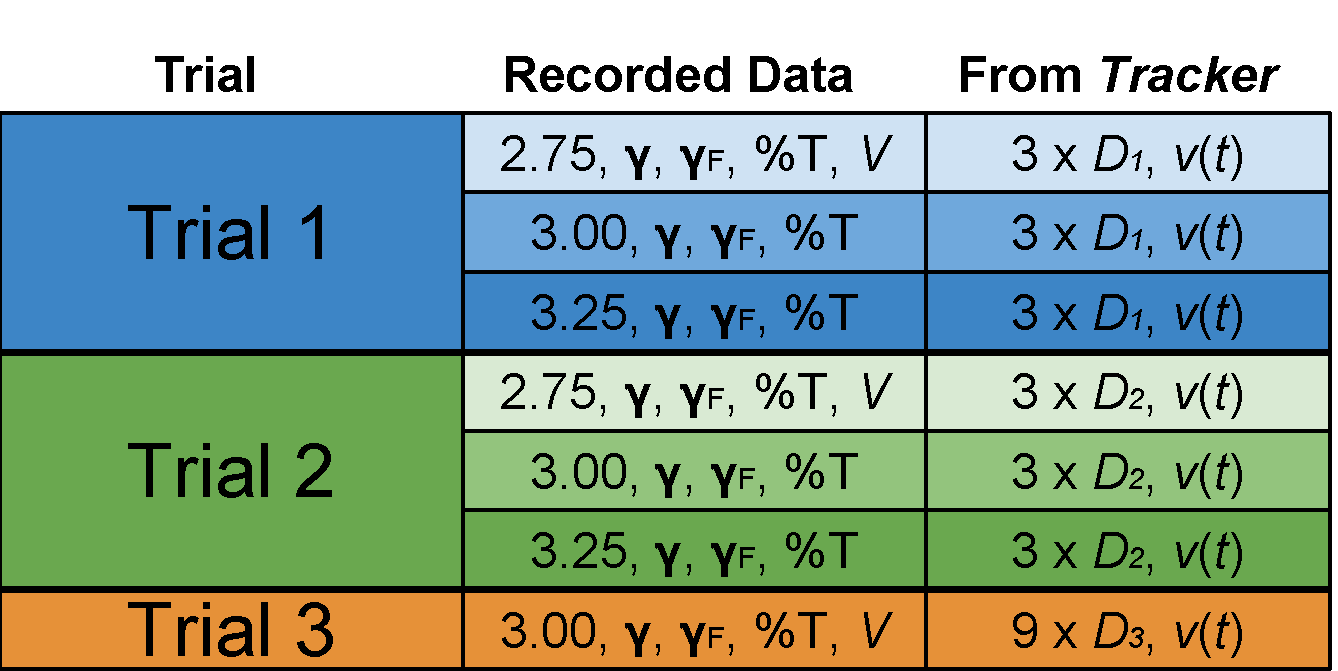
\includegraphics[scale=0.4]{datacollection.pdf}
	\caption{For each barrier ($2.75~\mathrm{mm}$, $3.0~\mathrm{mm}$, or $3.25~\mathrm{mm}$), the forcing accerlation ($\gamma$), the Faraday threshold acceleration ($\gamma_\mathrm{F}$), and the percentage of ``transmissions" (\%T) were recorded. The oil volume ($V$) was recorded at the beginning of each trial. From \textit{Tracker}, three measurements of the droplet diameter ($D_n$) were made along with the velocity of the droplet for every frame ($v(t)$).}
	\label{datacollection}
\end{figure}

These movies were then processed with \textit{Tracker}. \textit{Tracker} decomposes a video into multiple frames for the purpose of tracking an object in a video. By tracking the position of the object in every frame and knowing the time in between each frame ($\frac{1}{24}$ seconds), \textit{Tracker} estimates the velocity of the droplet at every frame. We also want to know the size of each droplet, so we measure the diameter of the droplet using a function in \textit{Tracker}. The diameter is measured multiple times in each movie, for reasons explained in \refSect{Sources of Error}.


From the volume of the oil $V$ and measurements taken of the tray, we can calculate the parameter $h$, which is defined as the height of the oil above the barrier. This was done by calculating the volume the ``space" inside the tray, which required accurate measurements of the tray components.\footnote{The function making this calculation can be found in the Appendix.}




%-------------------------
%        ANALYSIS
%-------------------------
\section{Analysis}


    \subsection{Tunneling vs. Oil Depth}
Our primary interest in this investigation was determining how tunneling was affected by depth of oil. The results are shown in \refFig{tbh}. The droplet never crossed near the value $h~=~1.0$, whereas it always crossed at a value $h~=~1.5$. In between, at a depth $h~=~1.25$, we have both transmissions and reflections at a rate that changes for every trial. If we consider the droplet diameter, we see that the plot suggests that the transmission coefficient increases depending on the diameter of the droplet.

\begin{figure}[h!]
	\centering
	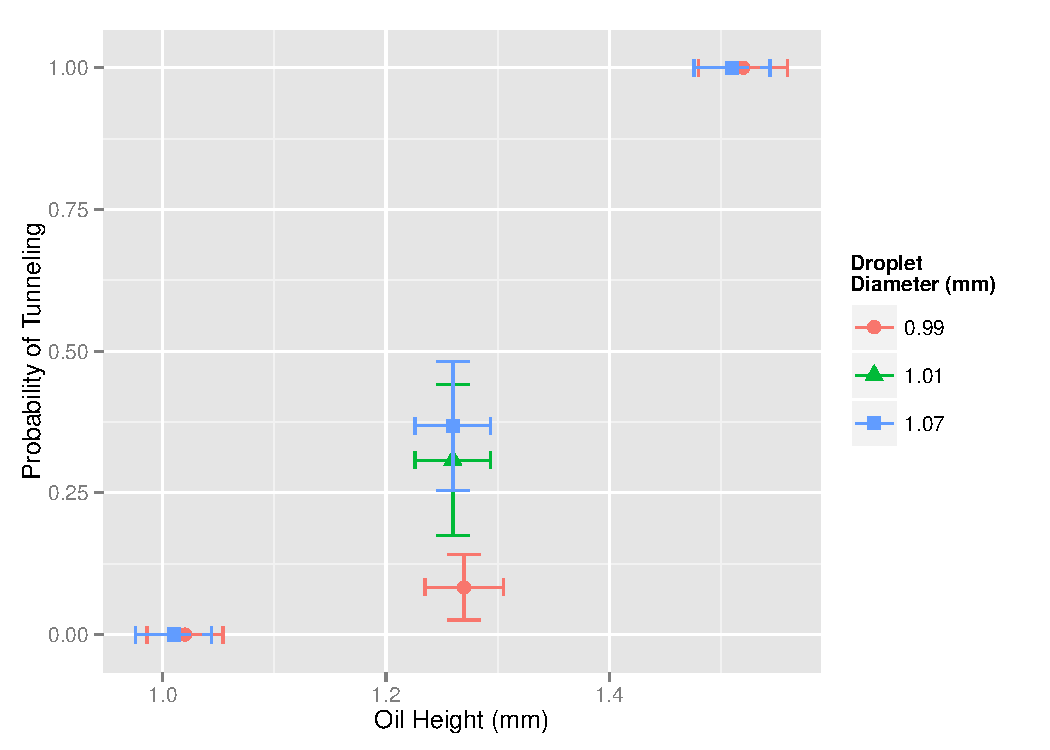
\includegraphics[scale=.9]{TunnelingProb.pdf}
	\caption{The proportion of transmissions for all collisions as a function of oil height above the barrier. Each color corresponds to a single trial for which the droplet was kept constant.}
	\label{tbh}
\end{figure}

    \subsection{Tunneling by Droplet Velocity}
Not every droplet barrier collision was ideal. Many times, the droplets approached at an angle or at different velocities which means that it is a little misleading to speak as if every collision was exactly the same. One way we can standardize collisions is by looking a perpendicular velocity at $5~\mathrm{mm}$ from the center of the barrier, as shown in \refFig{tvd}.

\begin{figure}[h!]
	\centering
	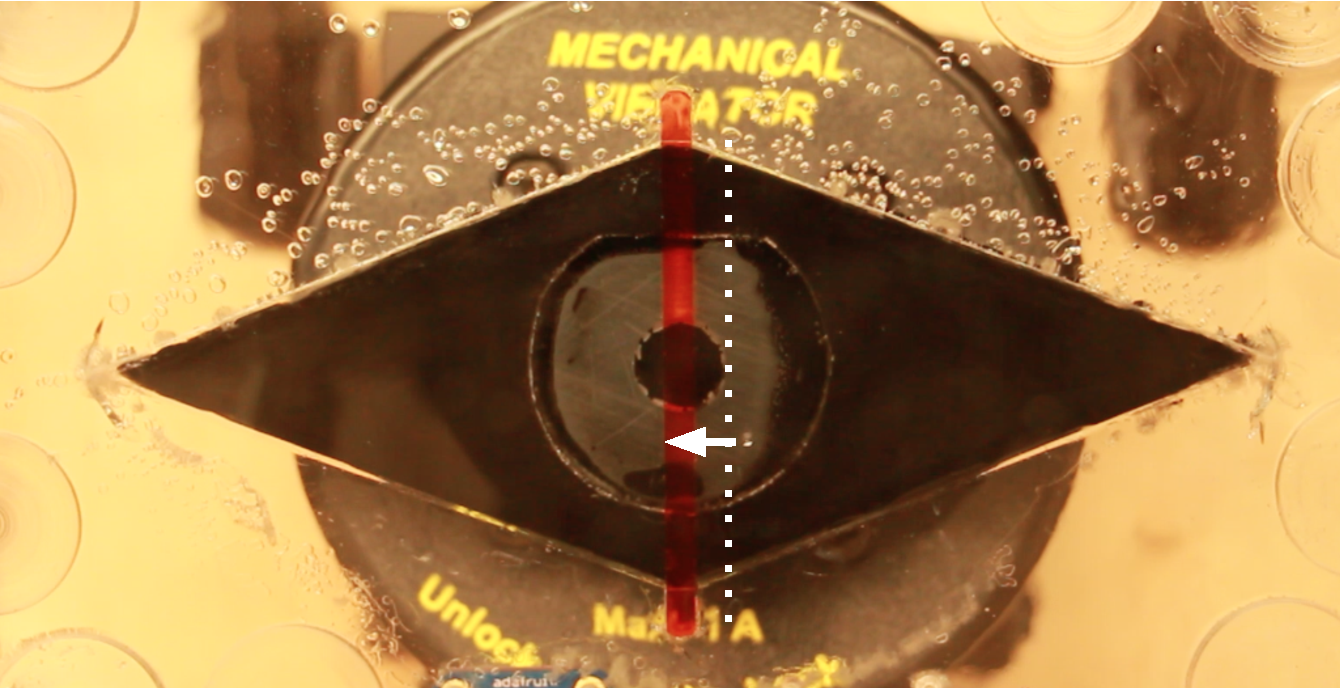
\includegraphics[scale=0.6]{TunnelingVDiagram.pdf}
	\caption{The image shows the point at which the perpendicular component of velocity was made, at $5~\mathrm{mm}$ from the middle of the barrier.}
	\label{tvd}
\end{figure}

We expect the perpendicular component of velocity to be important because it proved critical in the study of barrier width carried out in \ref{tunneling}, and because it's intuitive: if the droplet moves faster, it has greater momentum and is more difficult to stop. \refFig{vel} shows every collision for the middle barrier height, and the result of each interaction. 

\begin{figure}[h!]
	\centering
	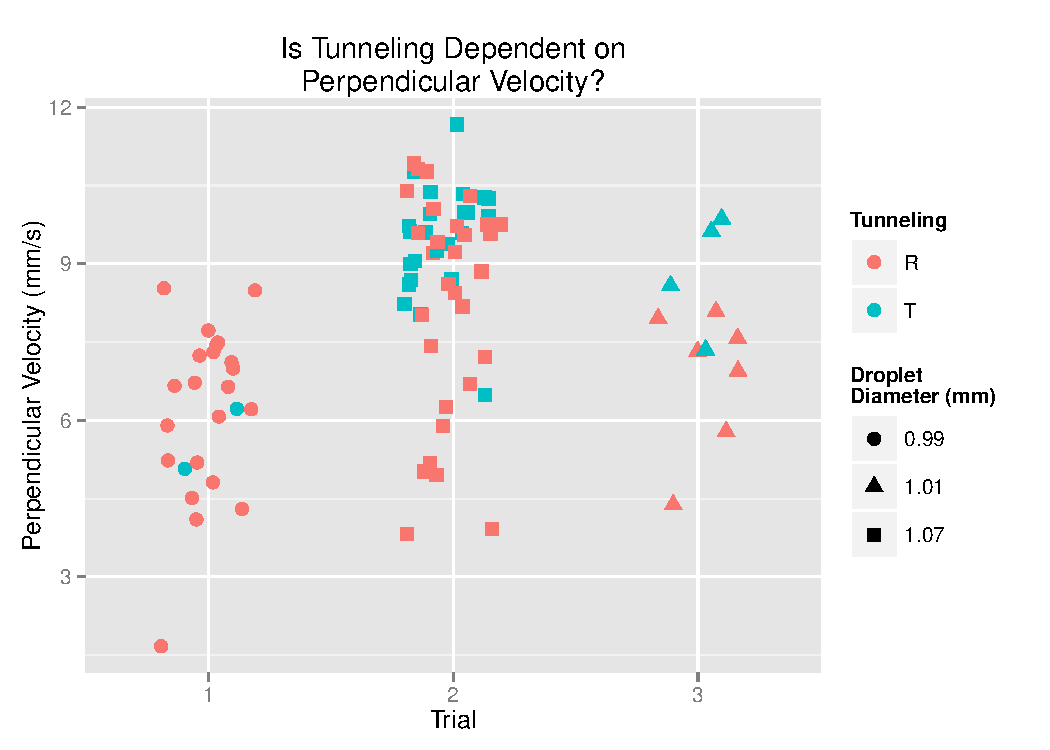
\includegraphics[scale=0.9]{Velocity.pdf}
	\caption{The result of each collision for the middle oil depth. The color represents the outcome of the collision (either transmission (T) or reflection (R)), and the shape represents the diameter of the droplet.}
	\label{vel}
\end{figure}

In trials 2 and 3, note that the majority of the droplets with the fastest perpendicular velocities are usually the ones that pass through the barrier, as expected. This does not seem to be the case for trial 1, for unknown reasons. 

%-------------------------
%       CONCLUSIONS
%-------------------------
%\section{Conclusions}


%-------------------------
%    SOURCES OF ERROR
%-------------------------
\section{Sources of Error}

    With a system like this one, sensitive to every tweak in any parameter, it's crucial to keep track of the errors so that we can consider the limitations these errors could have on our conclusions. Below I discuss the nature of the experimental errors associated with my measurements.
       
    \subsection{Droplet Diameter}
    The droplet diameter measurements were made using the \textit{Tracker} program. Knowing the length (in mm) of another object in the frame, in this case the length of the rhombus cutout inside the tray, we can measure the length of anything else in the frame (in mm). This works by finding the length in mm associated with each pixel in the frame, then knowing the width in pixels of the droplet, we can calculate it's length in mm.   
$$ 
\frac{\mathrm{length~of~rhombus~in~mm}}{\mathrm{length~of~rhombus~pixels}}= \frac{\mathrm{diameter~of~droplet~in~mm}}{\mathrm{diameter~of~droplet~in~pixels}} 
$$ 
Since each has a defined length, and because we can't resolve anything within that pixel, our error is associated with that measurement is at least the width of a pixel, usually around $\mathbf{0.08~\mathrm{\textbf{mm}}}$. There is also an error associated with the initial measurement of the rhombus in pixels, since it can be difficult to discern where exactly each point lies.

Additionally, the droplet does not remain a perfect sphere as it bounces. At the bottom of it's bounce, it will be squished and appear (from the top view) wider than usual, where at the moment of lift it will be less wide (from the top) than usual. Since the camera recording our data shoots at 24 frames per second, it's impossible to know at what point in the bounce the droplet is, so it's impossible to know when to measure the diameter of the droplet. For this reason we measured the diameter of the droplet in 3 frames per at each of the 3 barrier heights, and with the total of 9 separate measurements we averaged the results.\footnote{For the third trial in which only one barrier was used, the mm to pixel ratio was re-fit after three diameter measurements, in order to mimic the procedure of the first two trials.} Multiple measurements give us an associated standard error, which combined with the error due to pixel limitations, give us error bars. 

Our measurement procedure helped reduce the error associated with the changing size during a bounce. It also reduced the error associated with finding the exact mm to pixel ratio because within each trial, each barrier height was tracked separately so a new mm to pixel ratio was formed.  

    \subsection{Droplet Velocity}
The droplet velocity was measured using \textit{Tracker}. The error in this measurement can be attributed to the autotracker function, which automatically tracks the motion of the droplet using a built in algorithm. Autotracking is mostly spot on, but if left alone for a few thousand frames, the marker begins to drag behind. The error can be estimated to no more than 10 pixels, corresponding to $\mathbf{\pm~0.8~\mathrm{\textbf{mm/s}}}$.

    \subsection{Height of Oil}
The volume of oil was measured, before each trial, with a graduated cylinder marking every half milliliter. With measurements on the order of $18.0~\mathrm{mL}$, there was an associated error of $\mathbf{\pm~0.10~\mathrm{\textbf{mL}}}$. Then, oil was lost between each barrier adjustment, since pliers were inserted in the oil to pull each barrier out, and a little bit of oil remained on the barrier and on the pliers each time. The volume of fluid lost after each barrier replacement was estimated to be about 3 droplets of diameter $3.0~\mathrm{mm}$. This corresponds to a loss of $\mathbf{0.014~\mathrm{\textbf{mL}}}$ of oil after every change in barrier. 
Finally, the volume of the oil was used to estimate the height of the oil above the barrier. The elements in the tray were manufactured for this experiment, and were then measured using a device yielding an error of $\mathbf{\pm~0.03~\mathrm{\textbf{mm}}}$. 

For the height of the oil above the barrier, the above estimates provide us with an error on the order of about $\mathbf{\pm~0.35~\mathrm{\textbf{mm}}}$. The amount of fluid lost after each barrier replacement corresponds to a height decrease of $\mathbf{0.36~\mathrm{\textbf{mm}}}$ (for a barrier of the same size).

It's impossible to account for factors such as the amount of oil left in the graduated cylinder, or the oil that may have seeped into microscopic fractures inside the tray. We assume these systematic errors to remain relatively constant over the duration of the experiment. This means that the pattern of our results should remain about the same, even if the exact numbers are slightly off. 

    \subsection{Consistency of Memory}
The shaker's acceleration decayed the longer it ran which lead to changes in droplet behavior. This could be seen by the acceleration measured by the accelerometer, the acceleration decreased as the input signal remained constant. To counteract the changing acceleration, the amplitude of the signal was increased as such that it remained constant (as measured by the accelerometer) throughout the length of the experiment. After replacing each barrier, the Faraday threshold to that setup. As the amount of oil and the barrier height changed, the Faraday threshold also changed, so keeping the same input signal was not an option. Rather, in all experiments the \textit{memory} was kept constant, at around $98\%$ of the Faraday frequency. Because at different memories we see different droplet behaviors, a constant memory meant we could keep the behavior the same in all trials. 

    \subsection{Imperfect Droplet Motion}
The intent of the tray design was to create droplet trajectories such that their collisions were perpendicular to the length of the barrier. However, in practice, this was not the case. Trajectories tended to deviate to one side and impacted the barriers at an angle. Often, in situations in which the droplet was reflected, the trajectory would become a small limit cycle that would repeat for a couple of periods before diverging off in another path. 

The perpendicular velocity measurements were a work-around since they provide a more descriptive picture of each interaction. Even with this crutch though, the angled trajectories are a symptom of an imperfect setup. Though great care was taken to ensure that the tray was flat, it was impossible to adjust the mostly vertical direction of vibration to be perfectly vertical. When the oscillations are not exactly vertical, the oil inside the tray does not shake evenly, which leads to imperfect droplet motion. Rather than moving in a straight line until encountering a barrier of some sort, the droplet will slowly curl away from certain areas within the tray. Additionally, the tray in our setup was attached at a single point by a rod connected to the shaker. This could have lead to bending of the acrylic at the edges, since the tray was so big. A mechanical shaker, as detailed in \rf{shaker}, would provide a much better base than the smaller shaker used in this experiment. It also has the added benefit of shaking the entire tray at once, rather than just a single point. While the error due to this component cannot be measured numerically, it should be considered when drawing conclusions.




